\section{Introduction}
\label{chp:introduction} 

Computers, ranging from personal devices to embedded systems in automobiles, are essential in modern life and typically consist of hardware (physical components) and software (programs controlling the hardware). A key software component is the Operating System (OS), which acts as a bridge between hardware and software, with its kernel being the core program managing hardware details and enabling other programs to function~\cite{silberschatz2008-operatingsystemconcepts}. The Linux kernel, a Free/Libre/Open Source Software (FLOSS), exemplifies this by being highly customizable and widely used across various sectors, including Internet infrastructure and machine learning, making it a critical solution for real-world problems. Its adaptability and lack of licensing costs have made it central to the technology industry, supported by diverse stakeholders.

\subsection{The Linux kernel FLOSS ecosystem}

The Linux kernel project is structured into interconnected subsystems, analogous to neighborhoods in a city~\cite{wen2021-masterthesis}, each managed by maintainers who oversee contributions from developers. The \texttt{MAINTAINERS} file lists maintainers and their respective codebase portions. However, entries in the \texttt{MAINTAINERS} file often overlap and share code, forming clusters rather than isolated entities that more closely represent subsystems~\cite{corbet2021-subsystems}. The Linux community operates in a decentralized, global, and asynchronous manner, reflecting its distributed nature. Figure~\ref{fig:linux-subsystems} illustrates this complexity, showing an undirected graph of \texttt{MAINTAINERS} entries and their codebase overlaps, highlighting the interconnection of subsystems.


\begin{figure}[ht]
    \centering
    \begin{subfigure}[b]{0.3\textwidth}
        \centering
        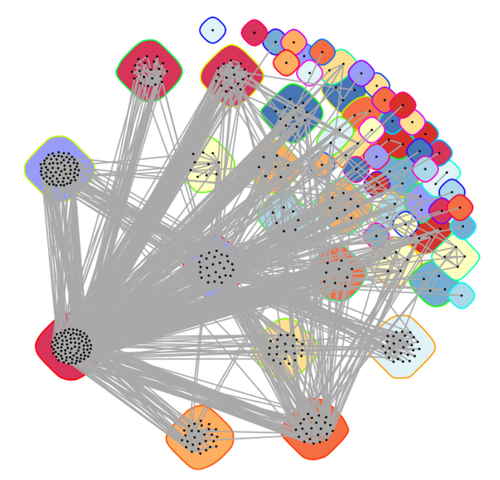
\includegraphics[width=1\textwidth]{images/linux-subsystems.png}
        \caption{Clusters of the \texttt{MAINTAINERS} file.\label{fig:linux-subsystems}}
    \end{subfigure}
    \begin{subfigure}[b]{0.3\textwidth}
        \centering
        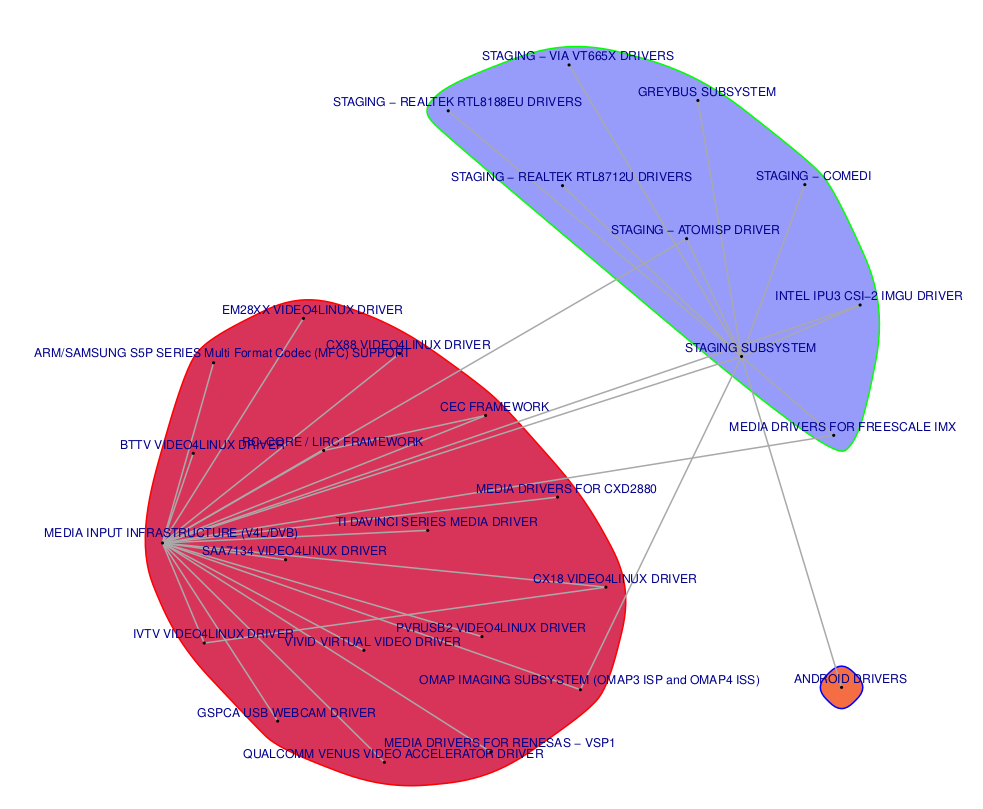
\includegraphics[width=1\textwidth]{images/media-subsystem.png}
        \caption{\textit{media} subsystem\label{fig:media-cluster}}
    \end{subfigure}
    \begin{subfigure}[b]{0.3\textwidth}
        \centering
        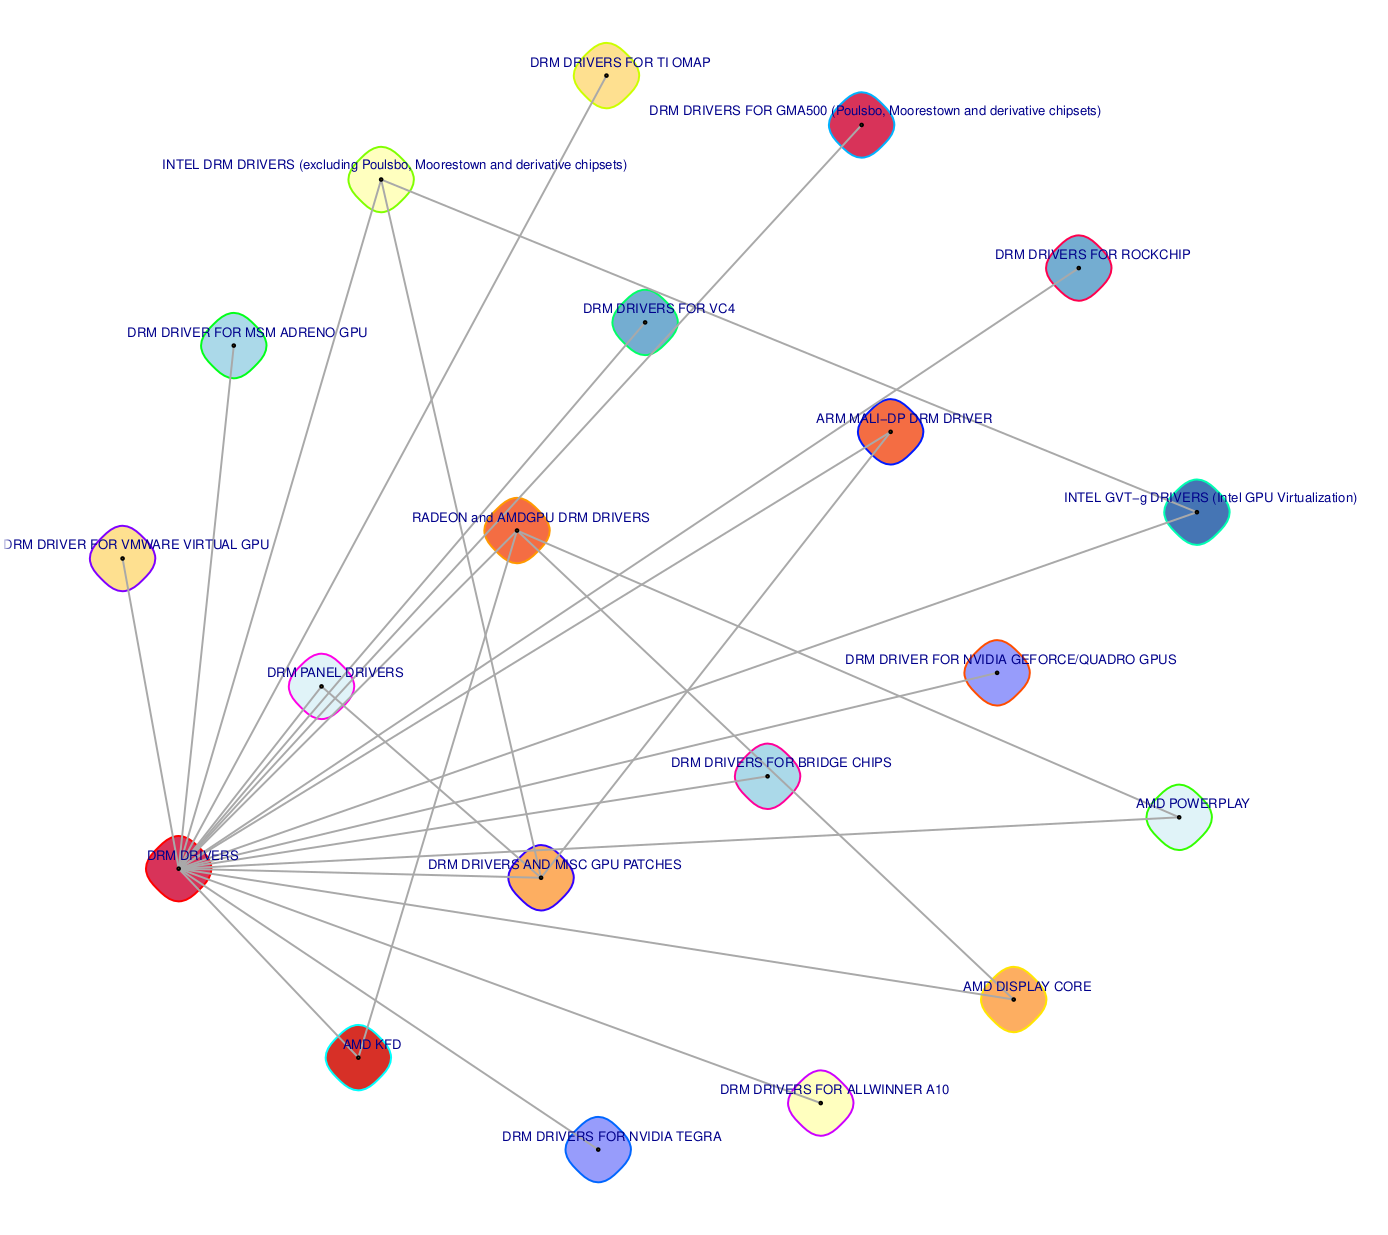
\includegraphics[width=1\textwidth]{images/drm-subsystem.png}
        \caption{\textit{DRM} subsystem\label{fig:drm-cluster}}
    \end{subfigure}
    \caption{Subsystems of the Linux kernel. \textit{Source} ~\cite{corbet2021-subsystems}.\label{fig:linux-clusters}}
\end{figure}

Despite their coupling, each subsystem has unique governance, maintainership models, and domain-specific characteristics. Figures~\ref{fig:media-cluster} and \ref{fig:drm-cluster} provide a closer look at the \textit{media} and \textit{DRM} subsystems, respectively, showcasing their distinct organizational structures. These examples underscore the diversity within the Linux kernel subsystems, even as they remain deeply interconnected~\cite{wen2021-masterthesis}.

\subsubsection{How the Linux kernel subsystems connect}

As mentioned, the Linux kernel project operates like a city divided into neighborhoods (subsystems), each governed by maintainers and supported by their ecosystems. These subsystems manage specific codebase portions within a hierarchical \textit{web of trust}, where upper levels delegate tasks to lower levels. Linus Torvalds, the creator of Linux, sits at the top as a \textit{benevolent dictator} \cite{corbet2014-4.4}, resolving disputes and overseeing the project. Despite this hierarchy, the structure is flatter than it seems, with most maintainers submitting pull requests\footnote{A request to merge changes made in one fork of a project into the original repository. Not to be confused with \textit{GitHub Pull-Requests}.} directly to Linus, bypassing mid-level maintainers \cite{corbet2017-patchflow}. While scalable, this model has led to inefficiencies, such as 44\% of contributions being ignored over the past decade \cite{rigby2014-peer-review}, causing frustration and wasted effort within the community.

\begin{figure}[ht]
    \centering
    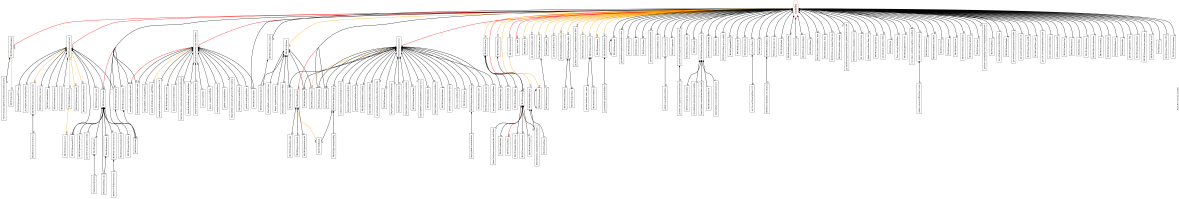
\includegraphics[width=1\textwidth]{images/treeplot-4.4-full-sm-fixed.png}
    \caption{Flow of changes from the Linux 4.4 development cycle as a tree plot showing the flat hierarchy of the development model (this figure is not supposed to be readable). \textit{Source}:~\cite{corbet2014-4.4}.\label{fig:4.4-hierarchy}}
\end{figure}

Subsystems function as independent projects with their own forks, synchronizing with the \textit{mainline} (Linus' tree) via pull requests. This decentralized model offers flexibility but creates dependencies on key maintainers, particularly Linus. Figure~\ref{fig:4.4-hierarchy} depicts the flat hierarchy of the Linux 4.4 development cycle, emphasizing Linus' central role and the ecosystem interconnection. Although this structure has driven Linux success, it exposes vulnerabilities, such as maintainer overload and reliance on critical individuals, which could threaten the project long-term sustainability.

\subsubsection{Patches and the Linux kernel development process}

At the heart of the Linux kernel development process is the \textit{patch}, a text document that describes changes between two versions of a source tree and represents a contribution to the project \cite{wen2021-masterthesis}. Similar to a git commit, a patch includes a code differential and a descriptive message but is formatted for email submission via mailing lists. Development, bug reporting, and discussions occur on these lists, with contributors submitting patches for review. Maintainers and the community provide feedback, leading to iterative revisions in a process known as the \textit{patch-reviewing process}. This back-and-forth ensures high-quality contributions \cite{palix2011-faults-linux}, and once a patchset (set of patches that comprise a contribution) is deemed ready, it begins its journey through the upstream (upper levels of Linux hierarchy) repositories.

\begin{figure}[ht]
    \centering
    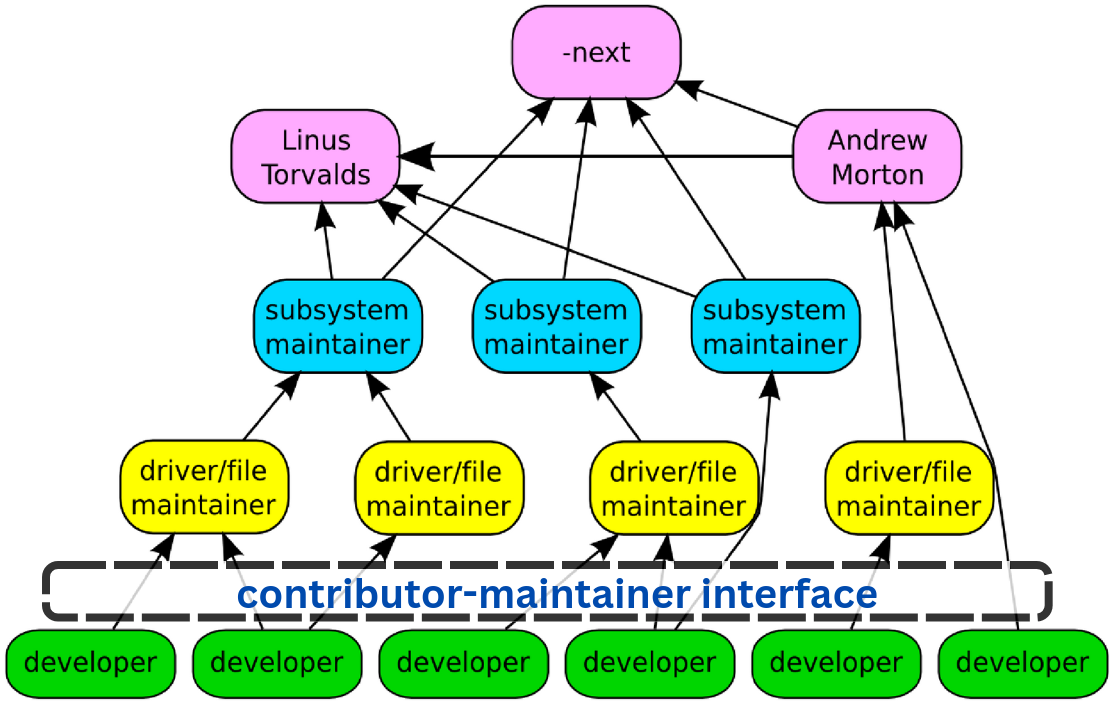
\includegraphics[width=0.4\textwidth]{images/patch-lifecycle.png}
    \caption{Patches flow into the \textit{mainline}. \textit{Source}:~\cite{gregkh2016-patches-carved}.\label{fig:patch-lifecycle}}
\end{figure}

Patches are first merged into the subsystem official repository, where maintainers have jurisdiction, and then progress up the hierarchy until they reach Linus Torvalds in the \textit{mainline} repository. Figure \ref{fig:patch-lifecycle} illustrates this flow, showing how patches move from contributors to the mainline. Along the way, \textit{Continuous Integration} (CI) practices, such as stabilization in \texttt{-next} branches, ensure changes do not destabilize the project. For example, the \textit{AMD DRM} subsystem uses the \texttt{amd-staging-drm-next} branch for this purpose.

Despite its effectiveness, the patch and email-based development process is considered outdated. \textit{Izquierdo-Cortazar et al. (2017)} \cite{izquierdo2017-review} argue for modernizing the review process, as mailing lists require proactive subscription and often face delivery issues. Tools like the Lore kernel archives and \textit{GitGitGadget} aim to address these challenges by providing real-time web access to mailing lists and enabling contributions via \textit{GitHub Pull-Requests}, respectively. These efforts highlight the need to adapt the Linux development model to contemporary standards while maintaining its collaborative and decentralized nature.

\subsubsection{The Linux kernel development model}

The Linux kernel development model encompasses a variety of \textit{workflows} that extend beyond technical functionalities, including practices like submitting patches to mailing lists, adhering to subsystem-specific rules, and following strict development cycles. These workflows are essential for maintaining the project structure and quality but also reveal bottlenecks that hinder efficiency. As noted by \textit{Corbet and Kroah-Hartman (2017)} \cite{corbet-gregkh2017-linuxreport}, tools are critical for managing the complexity of a project as large as Linux. For instance, git, created by Linus Torvalds in 2005, replaced the previous version control system and has since become indispensable for developers worldwide.

To address these bottlenecks, the Linux community develops tools ranging from official scripts like \texttt{get\_maintainers.pl} (finds patch recipients) to standalone projects like \texttt{b4} (fetches patches from archived mailing lists). Many developers also create personal scripts to solve specific issues, leading to duplicated efforts and a lack of systematic cataloging of solutions. Researchers involved in this project are actively developing FLOSS tools, such as the \textit{kworkflow}\footnote{\href{https://kworkflow.org}{https://kworkflow.org}} project and its subproject \textit{patch-hub}. These tools aim to unify solutions under a single interface, reducing inefficiencies and improving the overall development experience.

\subsection{Problem outline}

On one hand, the Linux kernel project steadily grows in size, complexity, and number of developers involved. On the other hand, we can name a few of the concerns about its development model detected by academia and practitioners:
(i) Scalability of the community and the workflows; 
(ii) Renewal of the workforce;
(iii) Key personnel that occupy critical roles and are often irreplaceable;
(iv) Waste of community effort and resources;
(v) Inefficient and outdated technologies that are at the core of the model;
(vi) \textit{Ad-hoc} solutions to workflow bottlenecks and duplication of work.


More severely, academic studies on the Linux project mostly detach from observing the practice and lack a proper investigation of these matters, carrying homogeneous and biased views~\cite{wen2021-masterthesis}. As a result, there are misleading conclusions from the academic that surface when contrasted with the perspective of the Linux community (\textit{Grey Literature}) and with the close observation of the practice (\textit{ethnographic case-studies}) \cite{wen2021-masterthesis}. We also point out that the ubiquity of \textit{ad-hoc} solutions to bottlenecks general to most Linux developers has an impact on the scalability of workflows and the workforce and compromises the project sustainability in the long term; therefore, in-depth academic research into the Linux ecosystem that unifies state-of-the-art and state-of-the-practice can lead to informed decisions on the development of critical tools that support the Linux umbrella project.
